\chapter{Project Design}

\section{Overview of the Design}

VisionSafe 360 is designed as a user-centered safety monitoring ecosystem for industrial and construction environments. The project focuses on converting raw safety observations into actionable intelligence to reduce incident response time and improve long-term preventive safety practices.

The primary objective is to manage four critical workplace risks: PPE compliance, fall events, unsafe proximity, and ergonomic hazards. The design distinguishes between \textbf{Emergency Response} (immediate action) and \textbf{Preventive Analytics} (long-term trends), ensuring that safety-critical events are surfaced with urgency while minimizing alert fatigue for long-term data. The design ensures a seamless integration between high-level oversight and rapid field-level intervention.

\section{System Architecture}

\textbf{Overall Architecture}

The system is structured as a modular, cross-platform architecture designed to support two distinct interaction environments:

\textbf{Control Room Environment (Web Dashboard):} Optimized for continuous situational awareness, detailed incident investigation, and administrative oversight.

\textbf{On-Site Response Environment (Mobile App):} Tailored for rapid alert reception, immediate acknowledgement, and field-level resolution logging.

\begin{figure}[H]
\centering
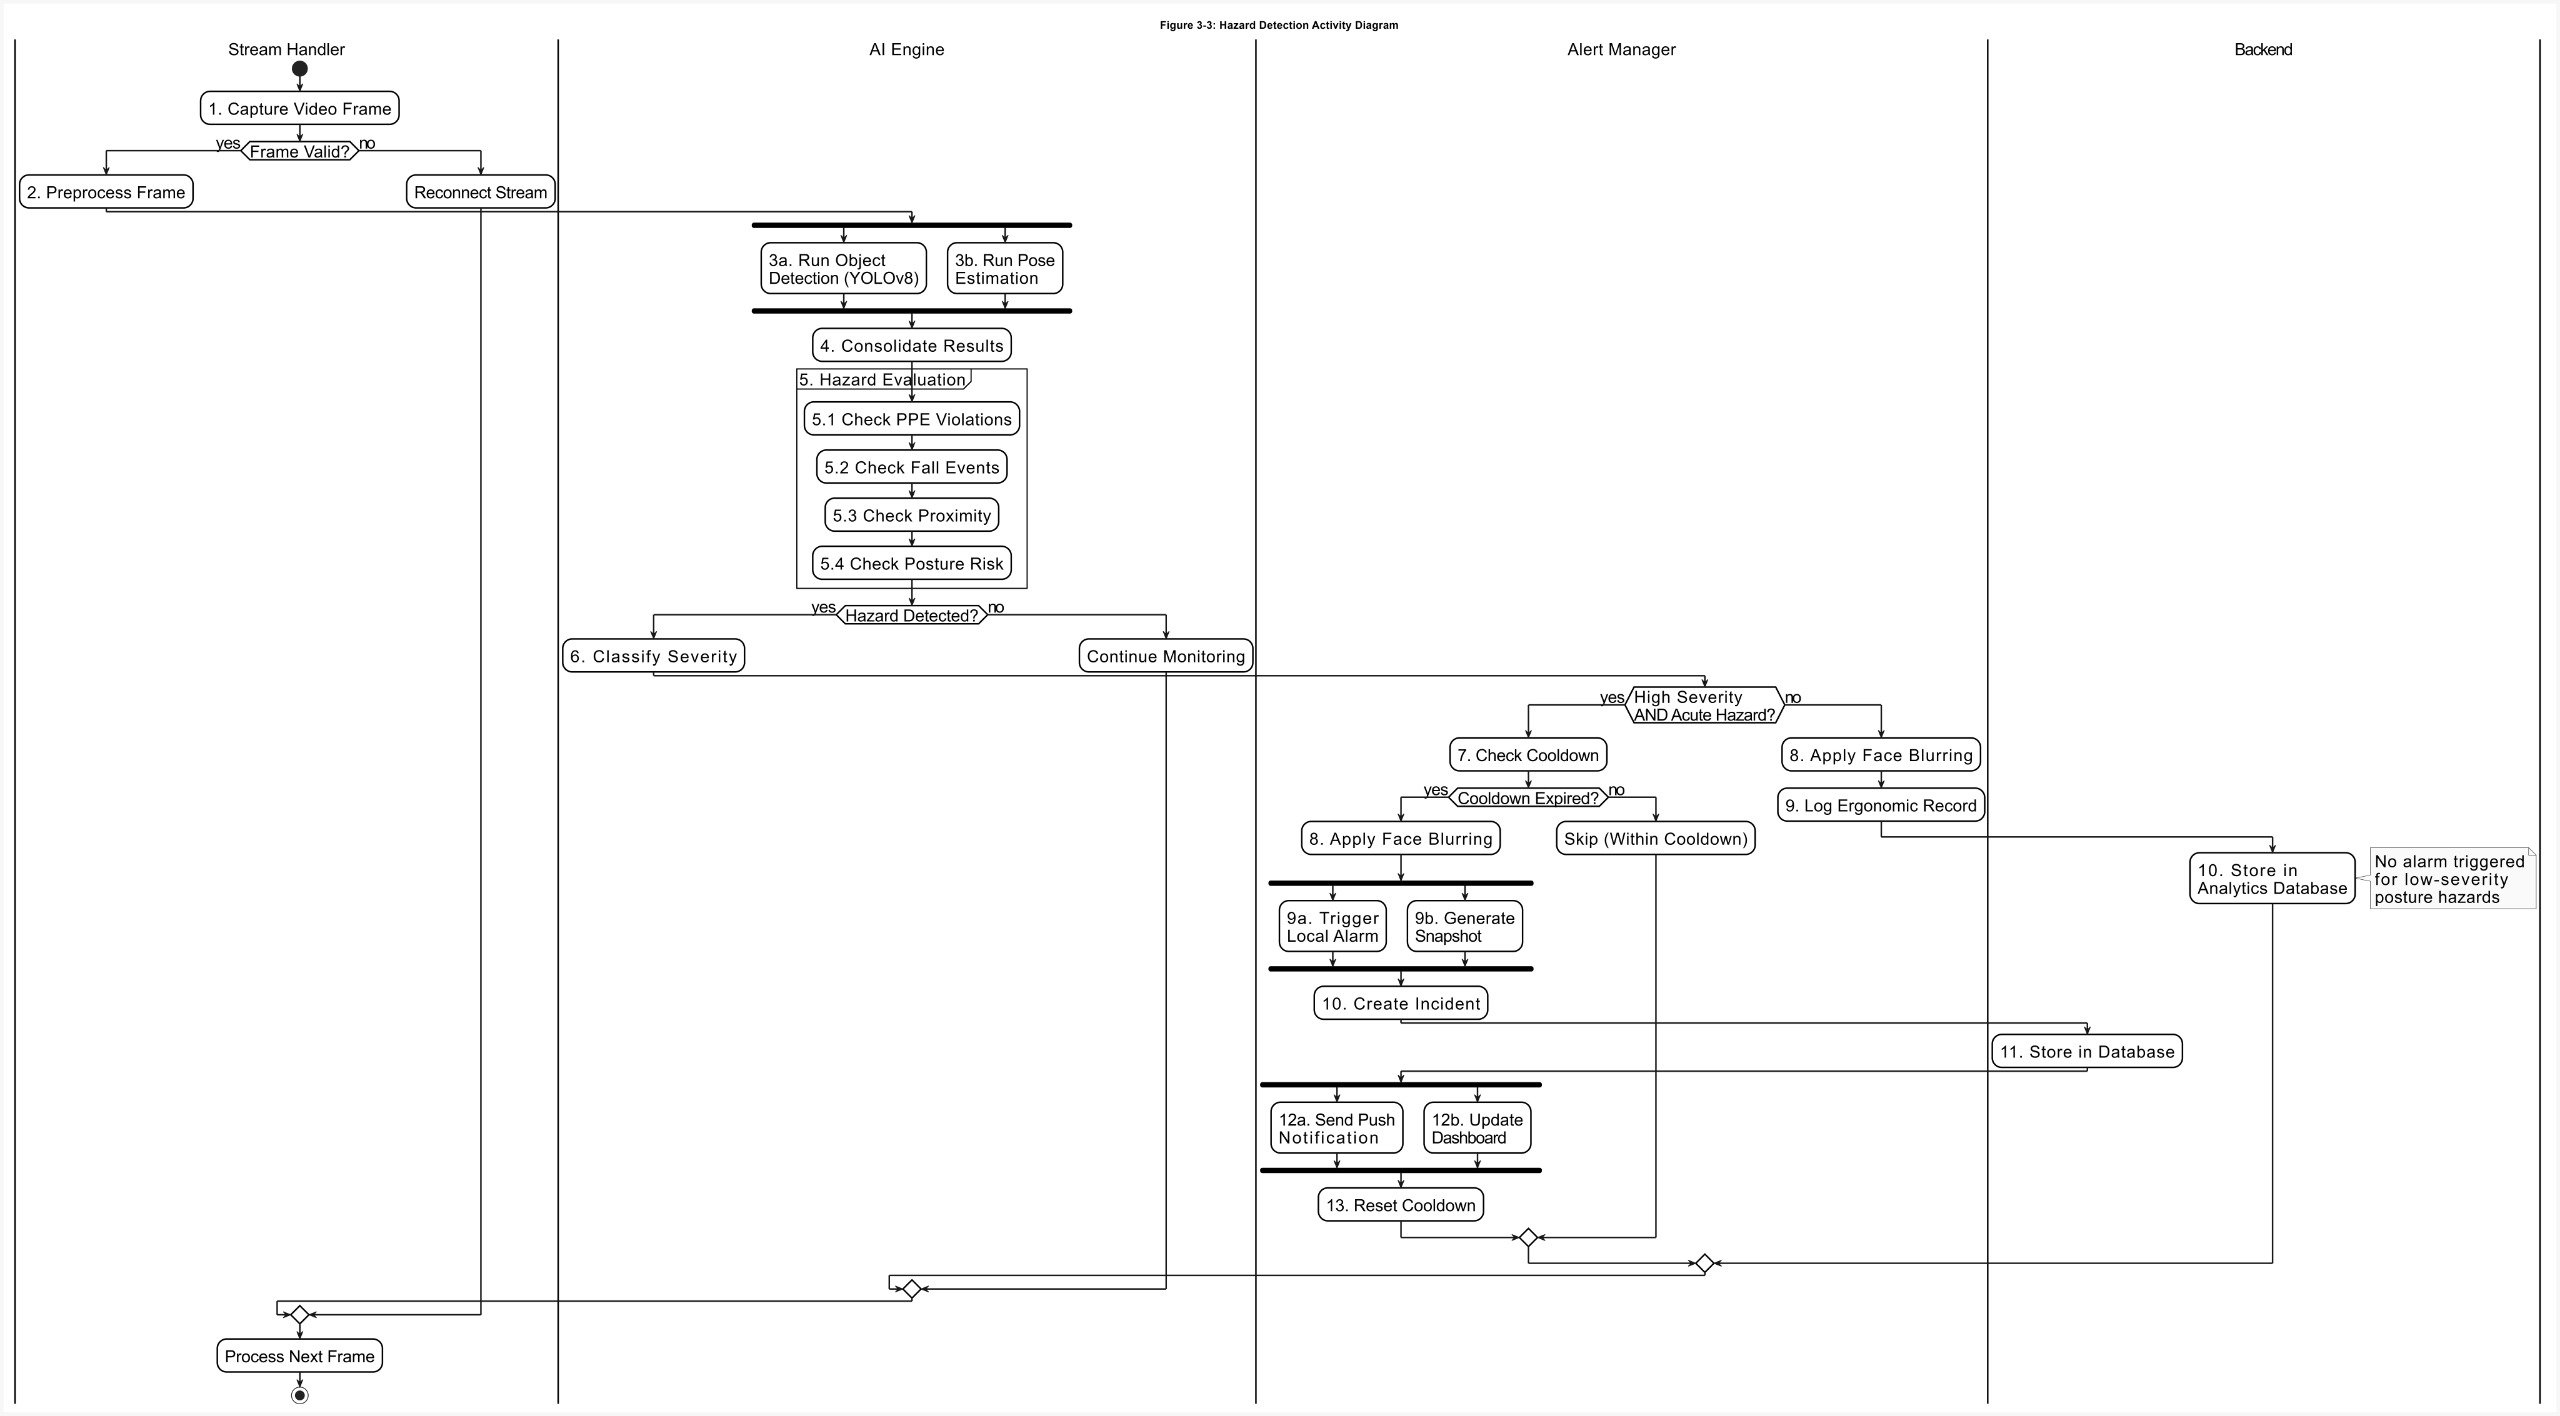
\includegraphics[width=0.95\linewidth,height=0.70\textheight,keepaspectratio]{images/img_017.jpeg}
\caption{System Architecture}
\end{figure}

\textbf{Component Roles and Interactions}

a. \textbf{Data Acquisition \& Processing:} Integrates camera feeds and AI models to detect safety breaches.

b. \textbf{Event Presentation Layer:} Translates system detections into human-readable summaries (type, severity, and location).

c. \textbf{Incident Lifecycle Manager:} Tracks events from the moment of detection through supervisor acknowledgement to final resolution.

d. \textbf{Analytics Engine:} Aggregates ergonomic and safety data into trend-based visual reports for long-term planning.

\section{Design Methodology}

The project utilizes an \textbf{Iterative, User-Centered Design (UCD) methodology}. This approach is essential for industrial safety systems where cognitive overload can lead to critical errors. The process involves repeated cycles of prototyping and refinement focusing on:

Information hierarchy and severity-based color coding.

Interface readability for control-room distances.

Mobile interaction efficiency for users in high-pressure field conditions.

Error prevention during high-impact actions like incident closure.

\section{Detailed Component Design}

The project design is modular, where each module corresponds to a distinct user task and interaction context:

\textbf{Monitoring Module (Web-centric):}

\textbf{Purpose:} Enables continuous scanning across multiple camera feeds.

\textbf{Design Details:} Features a stable grid layout, clear camera labeling, and a "Focus Mode" for high-priority streams.

\textbf{Emergency Incident Module (Dual-platform):}

\textbf{Purpose:} Surfaces urgent hazards requiring human intervention.

\textbf{Design Details:} Uses prominent visual cues (red/amber badges) and provides immediate access to incident snapshots.

\textbf{Incident Detail \& Evidence Module:}

\textbf{Purpose:} Supports quick confirmation and documentation of safety events.

\textbf{Design Details:} Displays anonymized evidence images, structured action logs, and a chronological timeline of the event lifecycle.

\textbf{Ergonomics Module (Preventive Analytics):}

\textbf{Purpose:} Supports the reduction of long-term musculoskeletal risks.

\textbf{Design Details:} Utilizes trend charts, exposure indicators, and zone-based heatmaps rather than intrusive alarms.

\section{UI/UX Design}

\textbf{A. Overview}

VisionSafe 360 delivers a unified experience where the \textbf{Web Dashboard} is optimized for investigation and the \textbf{Mobile App} is optimized for action. The design ensures consistent terminology, severity language, and navigation logic across both platforms.

\begin{figure}[H]
\centering
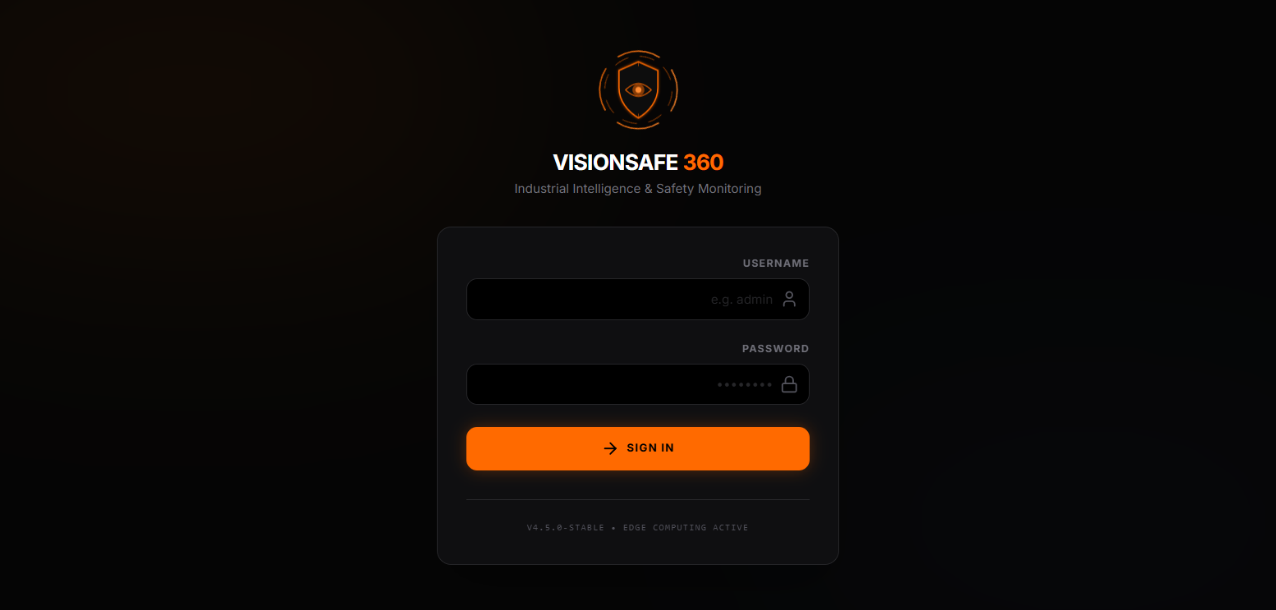
\includegraphics[width=0.95\linewidth,height=0.70\textheight,keepaspectratio]{images/img_018.png}
\caption{Web Dashboard Main Interface Layout}
\end{figure}

\begin{figure}[H]
\centering
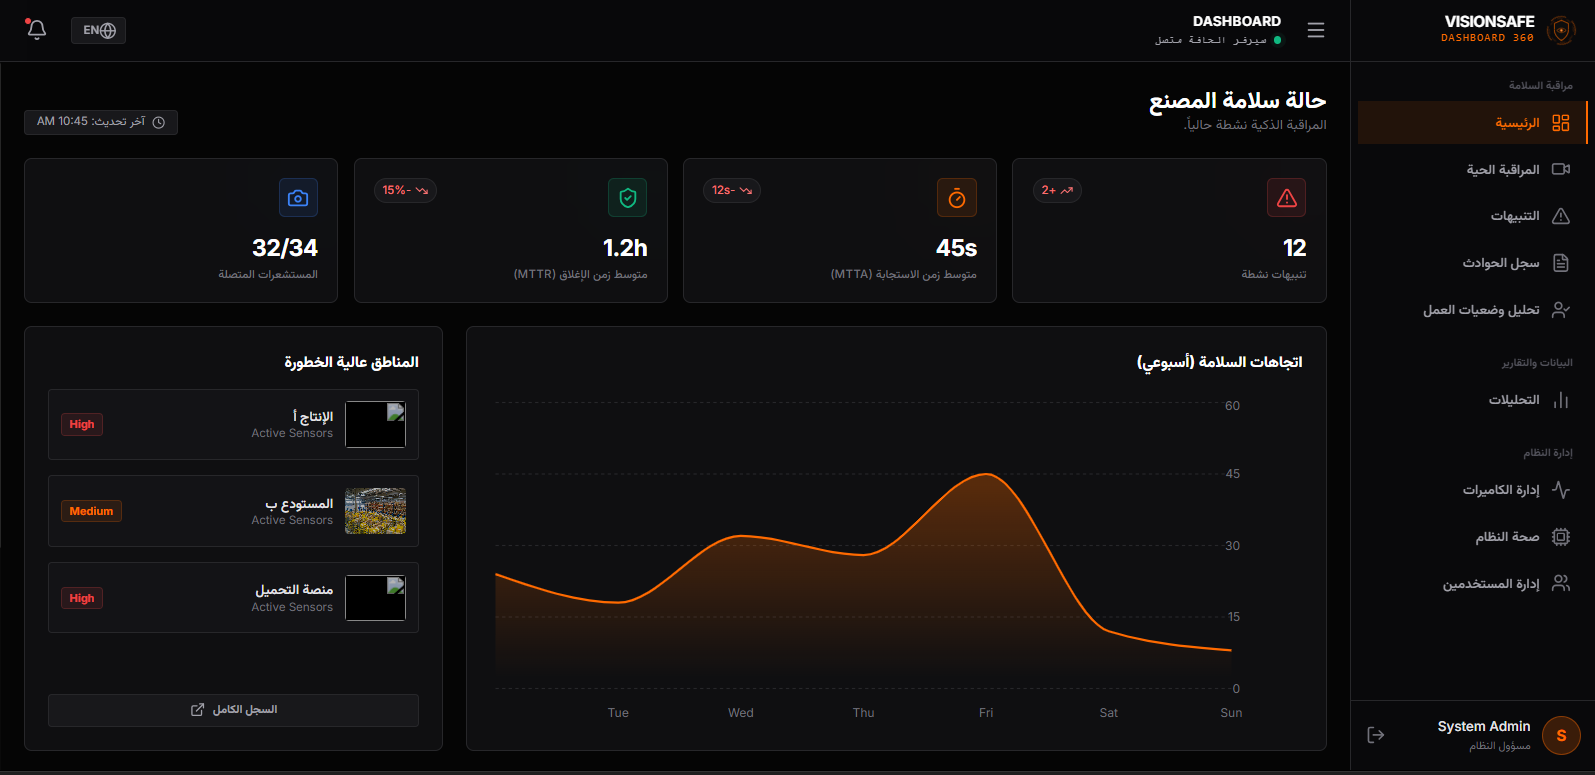
\includegraphics[width=0.95\linewidth,height=0.70\textheight,keepaspectratio]{images/img_019.png}
\caption{Web Dashboard Live Monitoring Interface}
\end{figure}

\begin{figure}[H]
\centering
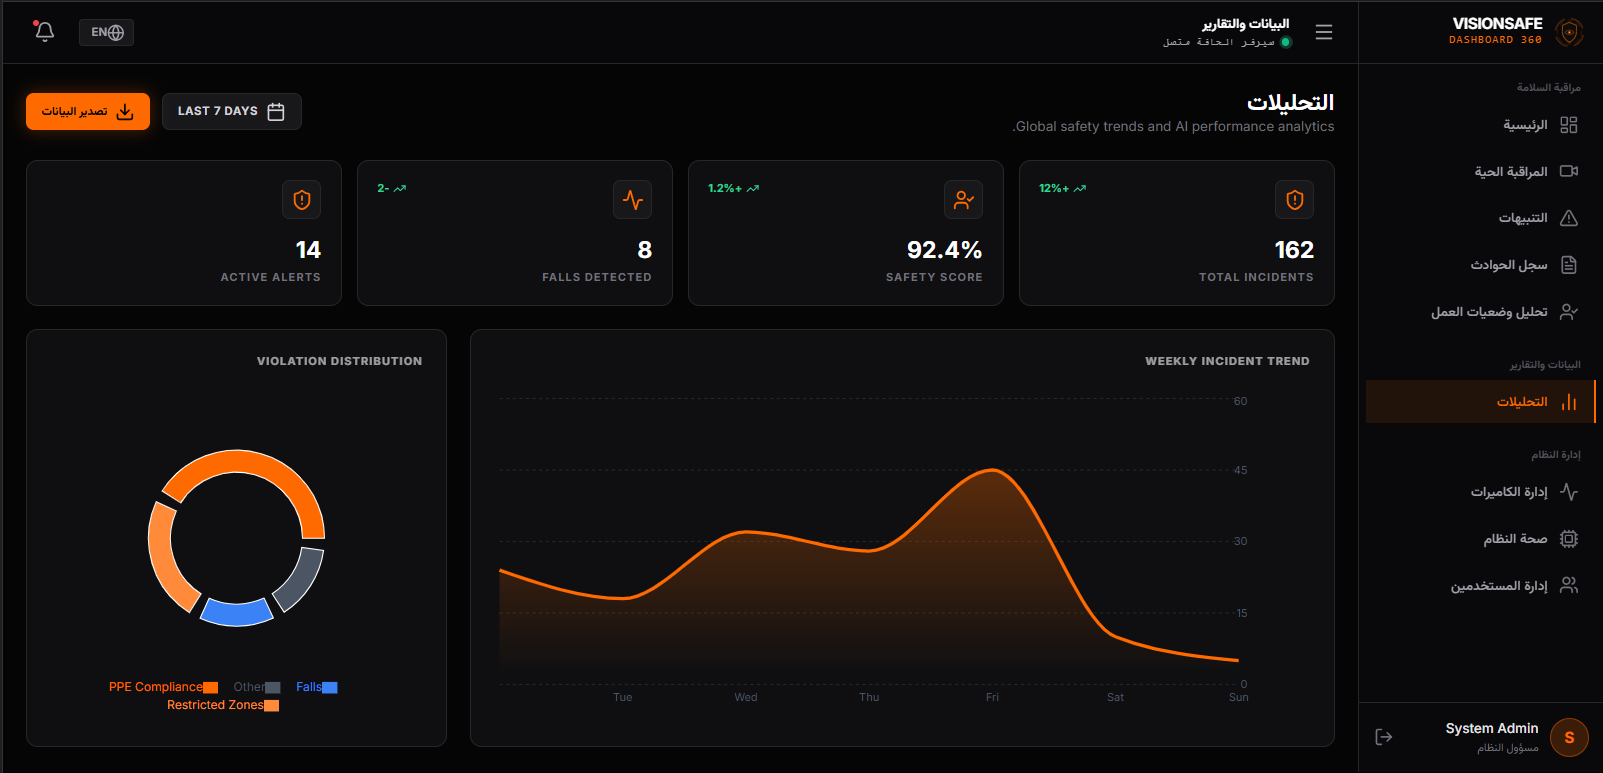
\includegraphics[width=0.95\linewidth,height=0.70\textheight,keepaspectratio]{images/img_020.png}
\caption{Web Dashboard Incident Interface}
\end{figure}

\begin{figure}[H]
\centering
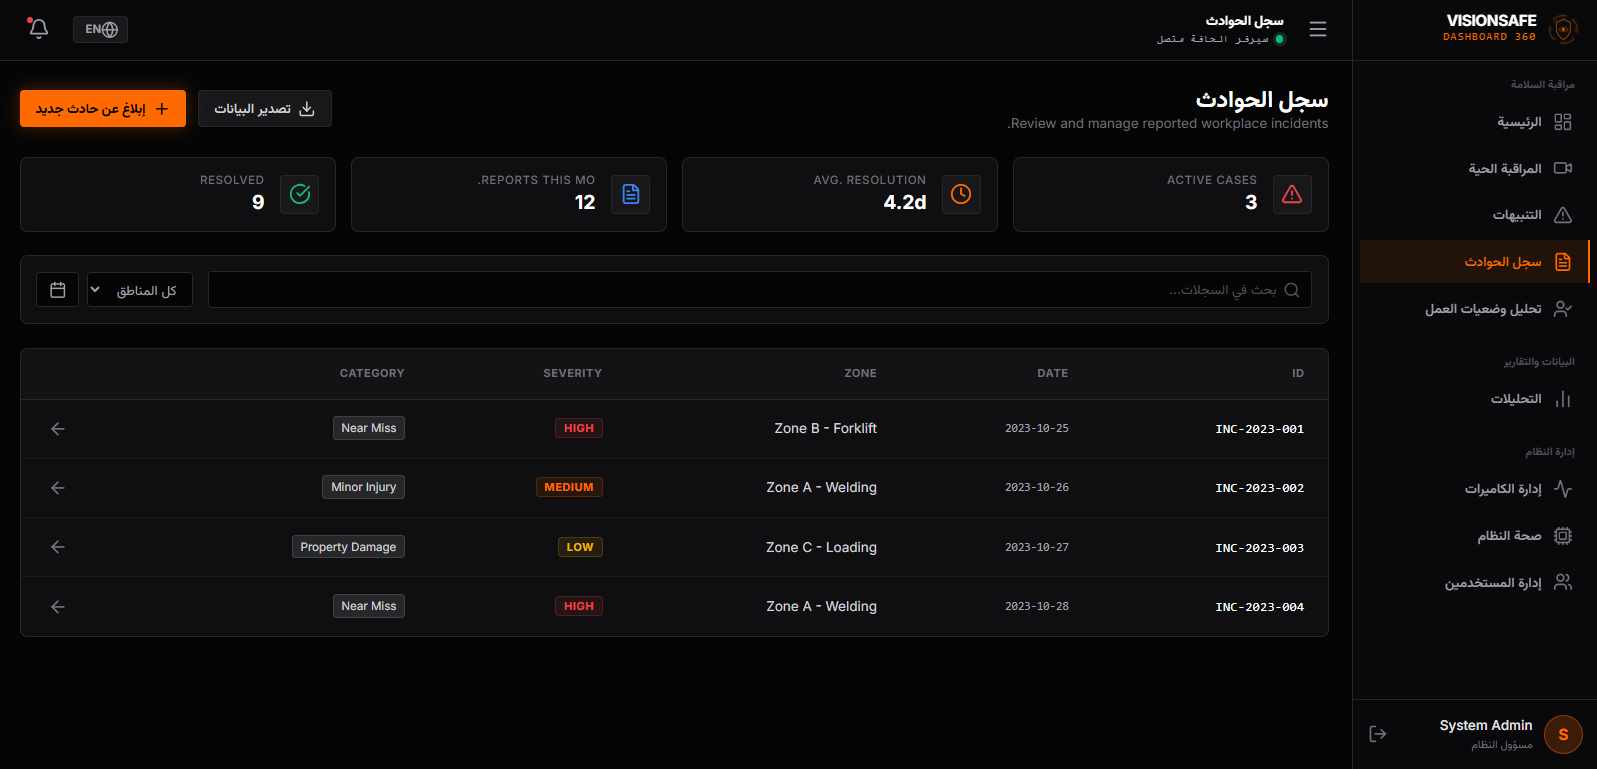
\includegraphics[width=0.95\linewidth,height=0.70\textheight,keepaspectratio]{images/img_021.png}
\caption{Web Dashboard Analytics Interface}
\end{figure}

\begin{figure}[H]
\centering
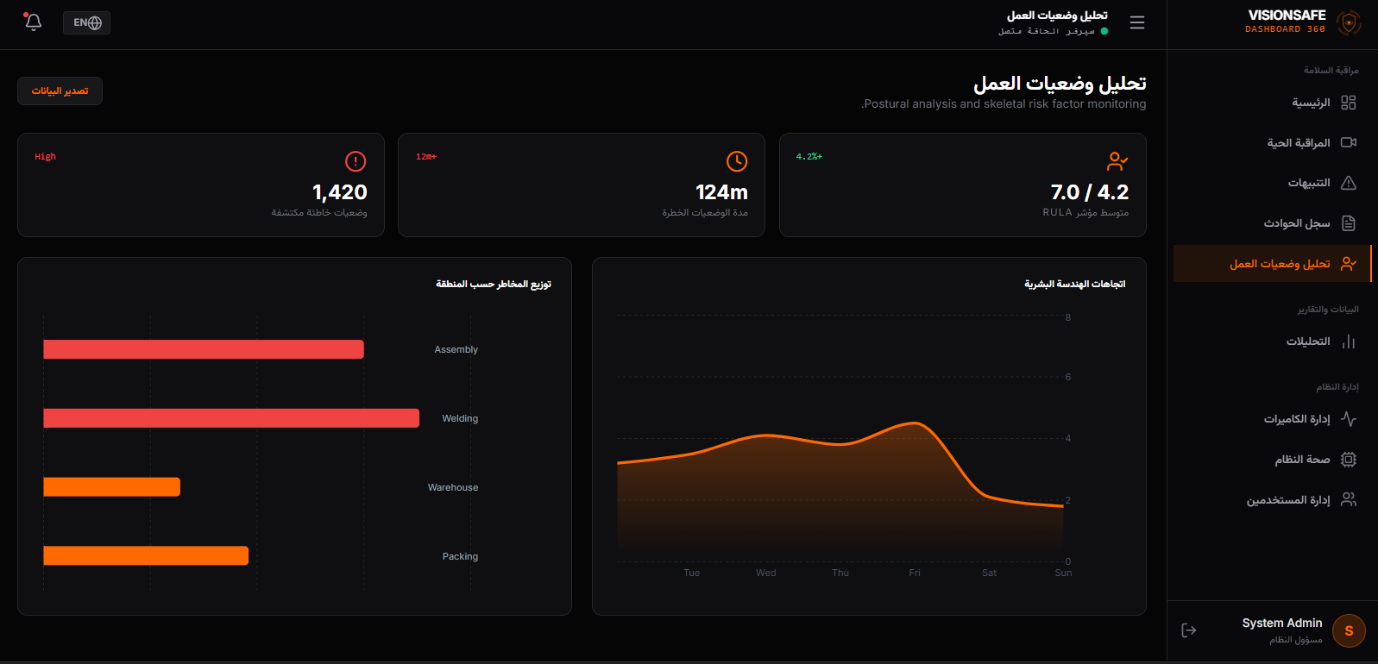
\includegraphics[width=0.95\linewidth,height=0.70\textheight,keepaspectratio]{images/img_022.png}
\caption{Web Dashboard Camera Management Interface}
\end{figure}

\begin{figure}[p]
\centering
\begin{minipage}[t]{0.45\linewidth}
	\centering
	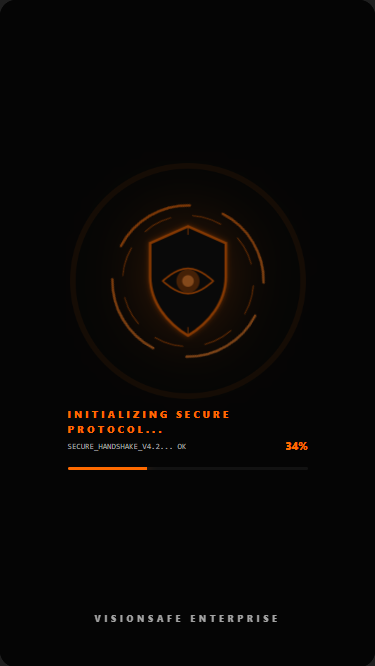
\includegraphics[height=0.34\textheight,keepaspectratio]{images/img_023.png}
	\captionof{figure}{Mobile Application Alert Overview}
\end{minipage}
\hfill
\begin{minipage}[t]{0.45\linewidth}
	\centering
	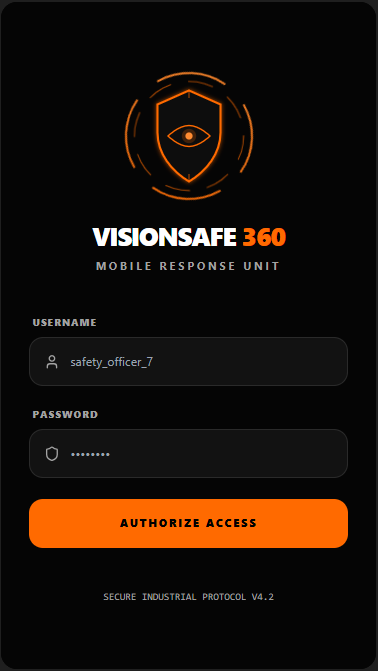
\includegraphics[height=0.34\textheight,keepaspectratio]{images/img_024.png}
	\captionof{figure}{Mobile Application Alert Details}
\end{minipage}

\vspace{0.8cm}
\begin{minipage}[t]{0.45\linewidth}
	\centering
	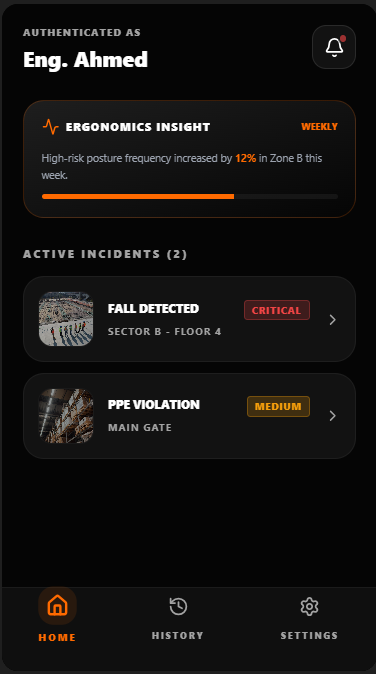
\includegraphics[height=0.34\textheight,keepaspectratio]{images/img_025.png}
	\captionof{figure}{Mobile Application Incident Acknowledgement}
\end{minipage}
\hfill
\begin{minipage}[t]{0.45\linewidth}
	\centering
	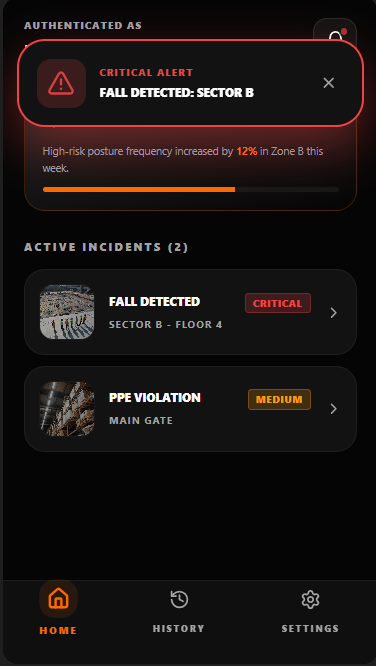
\includegraphics[height=0.34\textheight,keepaspectratio]{images/img_026.png}
	\captionof{figure}{Mobile Application Resolution Workflow}
\end{minipage}
\end{figure}

\begin{figure}[p]
\centering
\begin{minipage}[t]{0.45\linewidth}
	\centering
	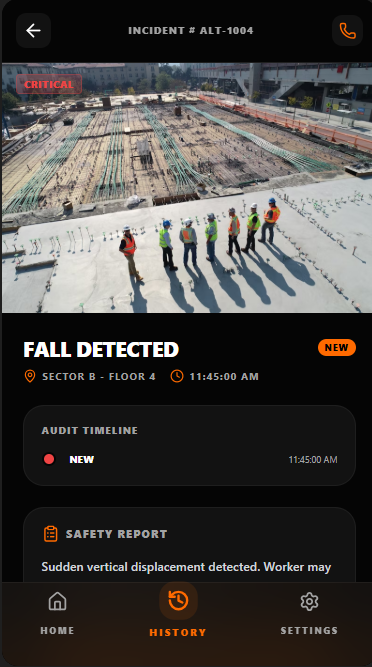
\includegraphics[height=0.34\textheight,keepaspectratio]{images/img_027.png}
	\captionof{figure}{Mobile Application Evidence View}
\end{minipage}
\hfill
\begin{minipage}[t]{0.45\linewidth}
	\centering
	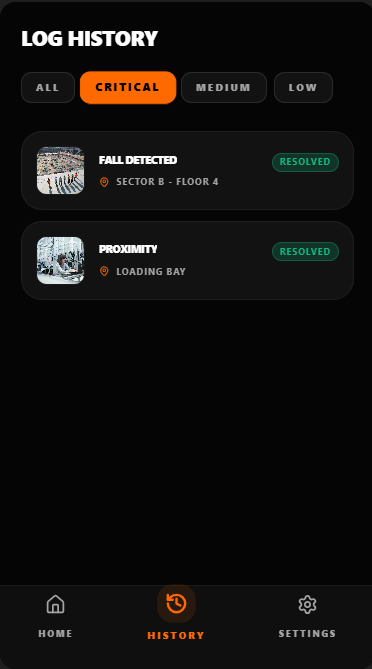
\includegraphics[height=0.34\textheight,keepaspectratio]{images/img_028.png}
	\captionof{figure}{Mobile Application Camera Status}
\end{minipage}

\vspace{0.8cm}
\begin{minipage}[t]{0.45\linewidth}
	\centering
	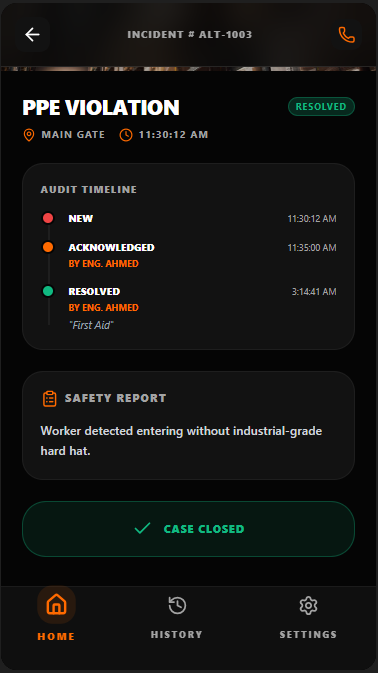
\includegraphics[height=0.34\textheight,keepaspectratio]{images/img_029.png}
	\captionof{figure}{Mobile Application Notifications}
\end{minipage}
\hfill
\begin{minipage}[t]{0.45\linewidth}
	\centering
	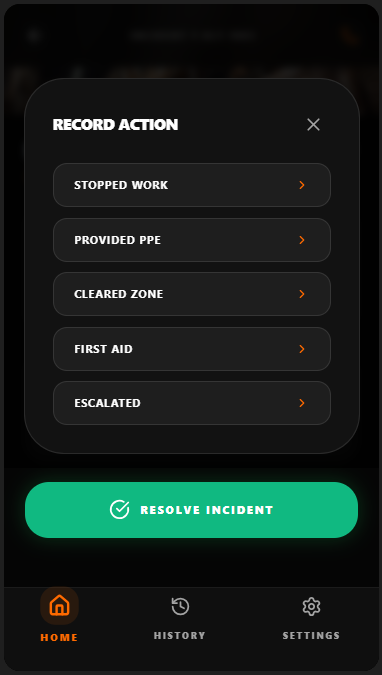
\includegraphics[height=0.34\textheight,keepaspectratio]{images/img_030.png}
	\captionof{figure}{Mobile Application Ergonomic Alert}
\end{minipage}
\end{figure}

\begin{figure}[p]
\centering
\begin{minipage}[t]{0.62\linewidth}
	\centering
	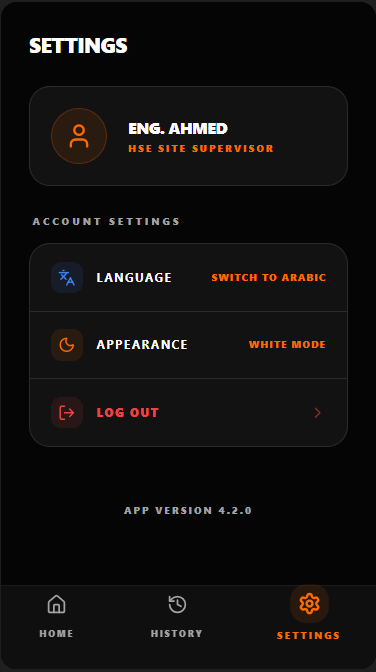
\includegraphics[height=0.60\textheight,keepaspectratio]{images/img_031.png}
	\captionof{figure}{Mobile Application Interface for Field Alerts}
\end{minipage}
\end{figure}

\textbf{B. User Interaction}

\textbf{The application ecosystem allows users to:}

Monitor multiple camera views and quickly focus on a specific feed.

Review emergency incidents with clear severity and location context.

Acknowledge incidents via mobile or web to confirm awareness and ownership.

Resolve incidents by recording corrective actions for audit purposes.

\textbf{Outputs are delivered through:}

\textbf{Incident Cards:} Summarizing type, severity, location, and timestamp.

\textbf{Visual Evidence:} Anonymized snapshots for rapid incident confirmation.

\textbf{Trend Dashboards:} Summary indicators and charts for long-term analysis.

\textbf{C. Design Principles}

\textbf{Simplicity:} Reducing cognitive load through clean layouts and minimal steps for critical actions.

\textbf{Clarity and Hierarchy:} Prioritizing urgent hazards while keeping secondary details available but not dominant.

\textbf{Accessibility:} High contrast, readable typography, and non-color-only severity cues (using icons and text).

\textbf{Error Prevention:} Confirmation dialogs for destructive actions and clear system-state indicators (e.g., offline camera).

\section{Workflow Design}

\textbf{A. Emergency Incident Workflow}

This workflow ensures that every detected hazard is accounted for by a human supervisor.

\textbf{Detection:} AI identifies a hazard and triggers an alert.

\textbf{Notification:} Alert appears on the Web Dashboard and the Mobile App simultaneously.

\textbf{Acknowledgement:} A supervisor confirms ownership via the mobile device.

\textbf{Resolution:} The supervisor records the corrective action taken to close the incident.

\textbf{B. Ergonomics Workflow}

\textbf{Passive Monitoring:} Ergonomic risks are logged as data points without immediate alarms.

\textbf{Trend Analysis:} HSE Managers review cumulative data on the Web Dashboard weekly/monthly.

\textbf{Strategic Intervention:} Decisions are made based on high-risk zones or recurring posture issues.

\section{Database Design (Conceptual)}

\textbf{A. Overview}

The database is structured to support the core UX requirements: traceability, accountability, and reporting. It ensures that data remains consistent across the Web and Mobile interfaces.

\textbf{B. Table Descriptions}

\textbf{Users \& Roles:} Manages identity and access scope (Admin, Manager, Supervisor).

\textbf{Cameras:} Stores camera metadata and location tagging for UI labeling.

\textbf{Incidents:} Core table tracking hazard types, severity, snapshots, and lifecycle status.

\textbf{Ergonomic Records:} Stores posture risk summaries and exposure indicators for analytics.

\textbf{Action Logs:} Maintains an audit trail for every acknowledgement and resolution action.

\begin{figure}[H]
\centering
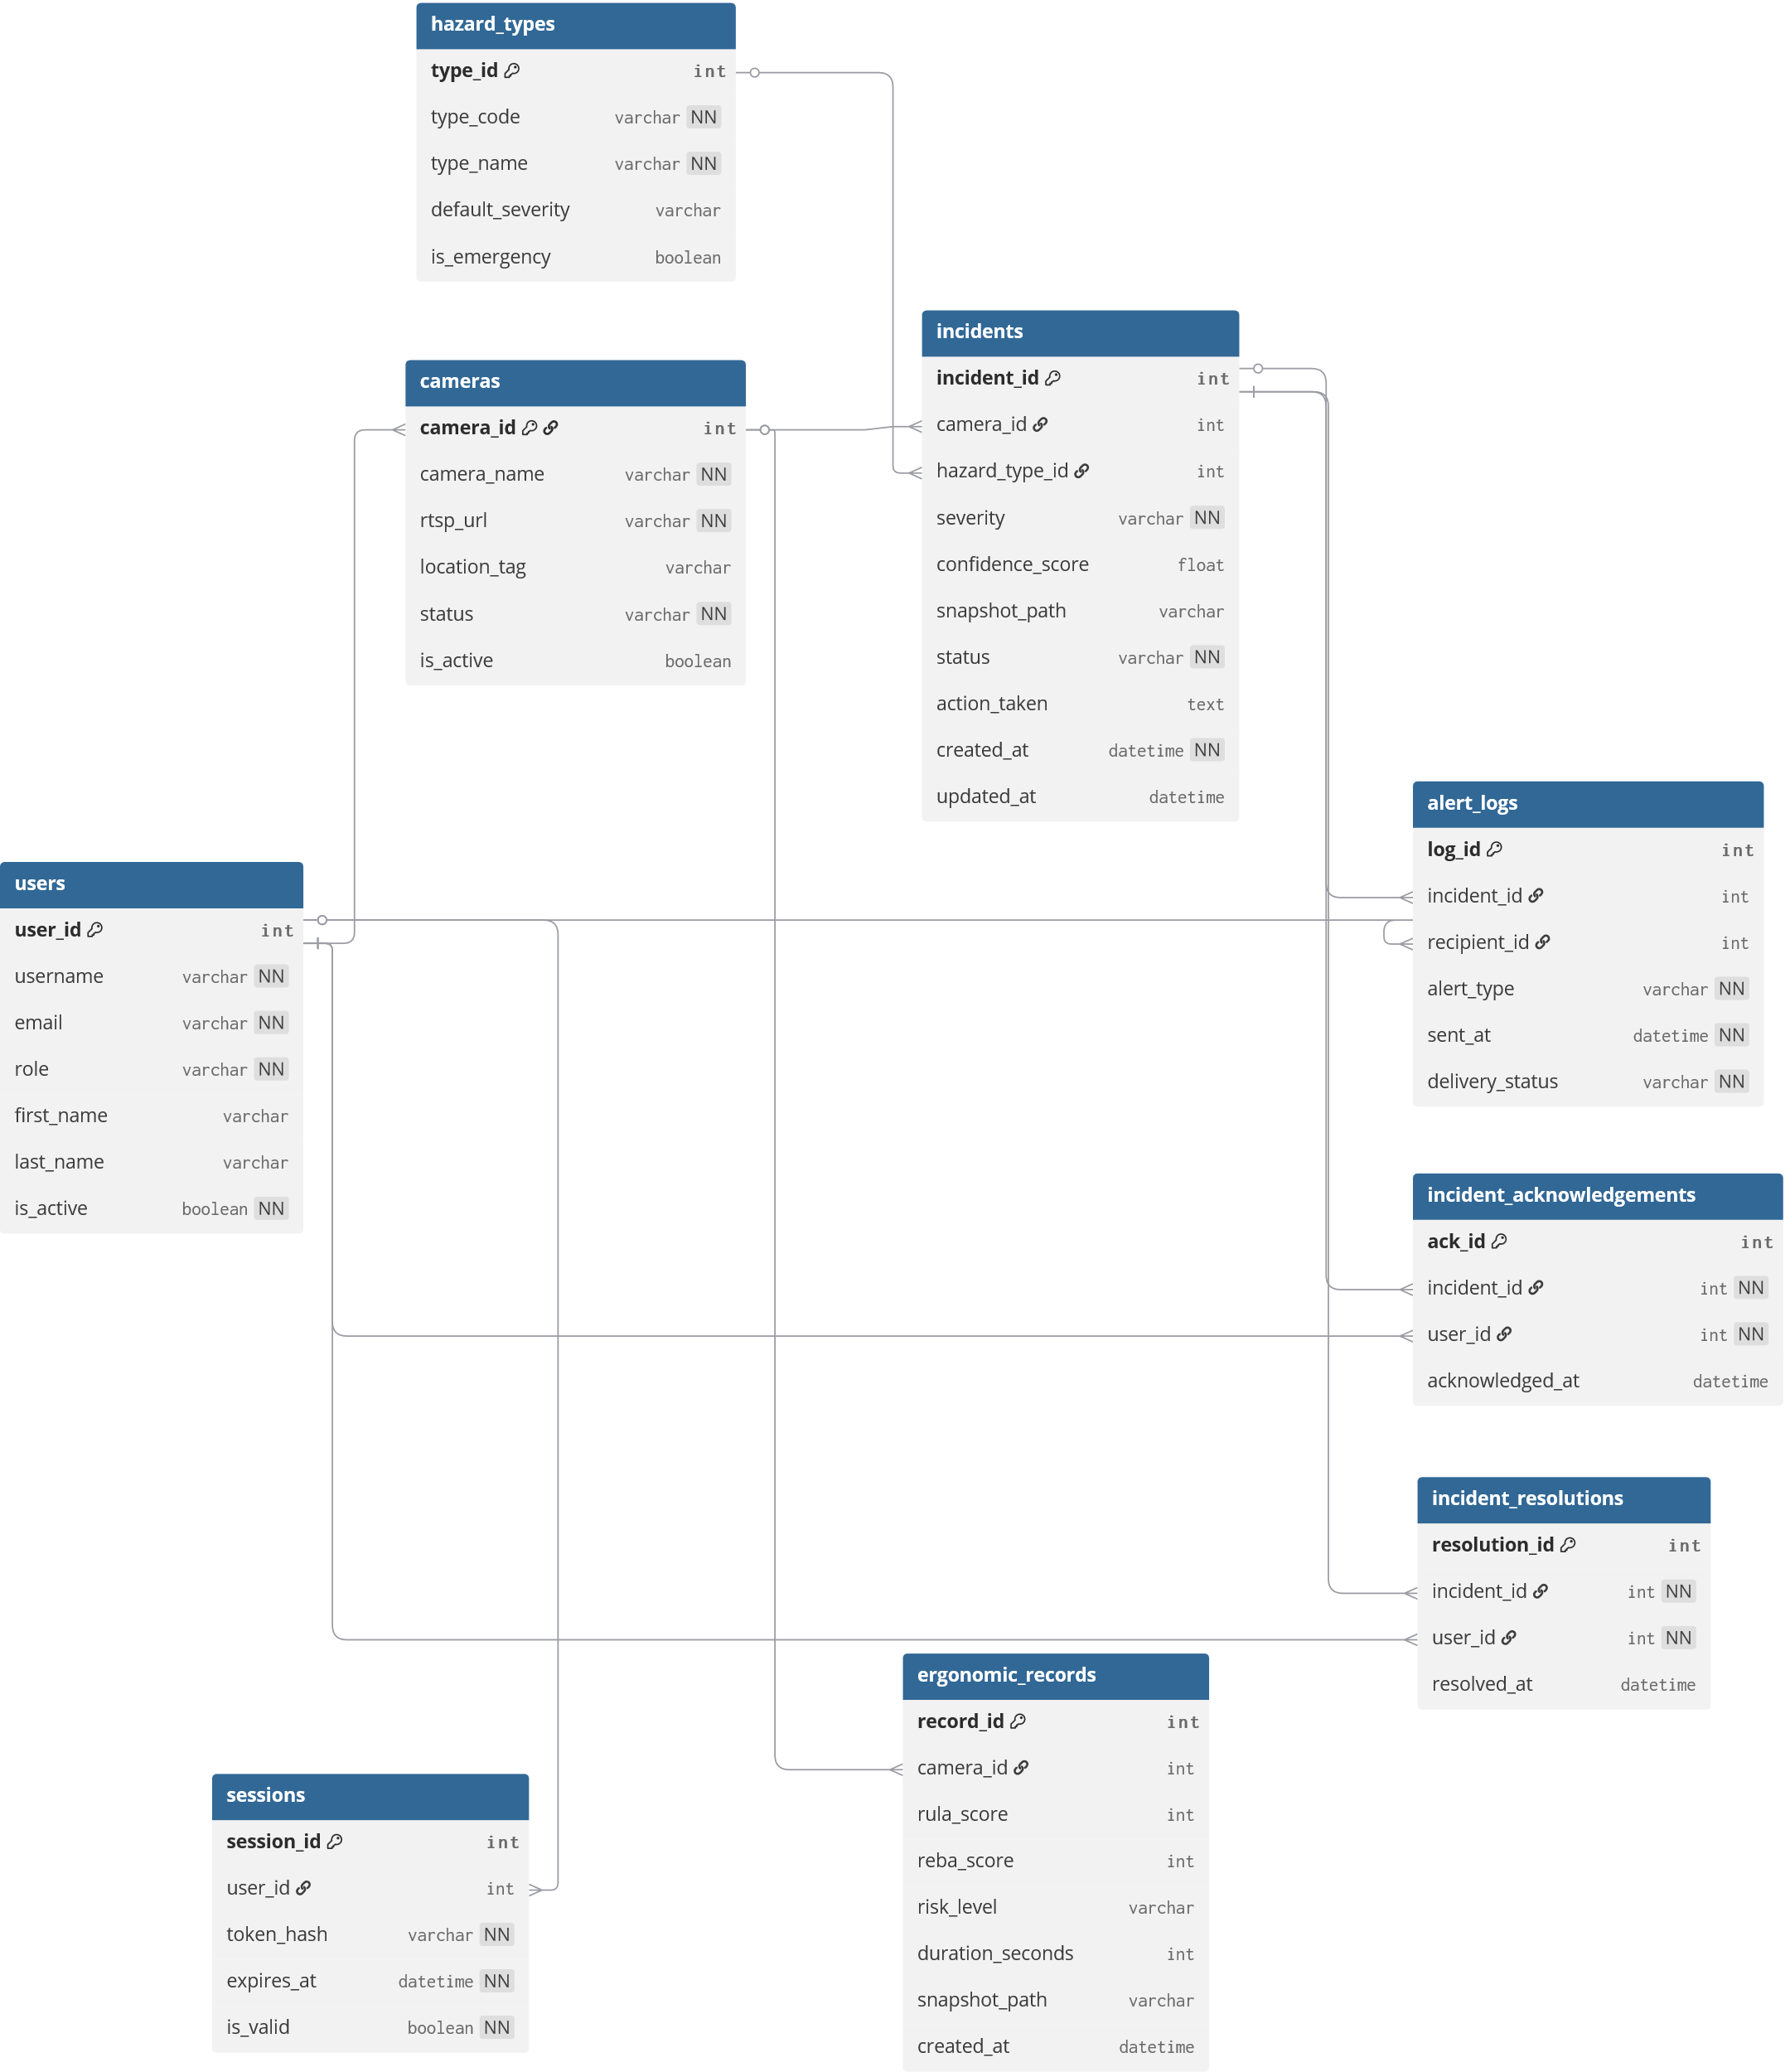
\includegraphics[width=0.95\linewidth,height=0.70\textheight,keepaspectratio]{images/img_032.png}
\caption{Entity-Relationship Diagram (ERD)}
\end{figure}

\section{Design Constraints}

a. \textbf{Operational Context:} Industrial environments introduce noise and distractions, requiring high-visibility UI.

b. \textbf{Monitoring Duration:} Visual design must minimize eye strain for control-room operators during long shifts.

c. \textbf{Device Diversity:} The design must remain usable on large desktop displays and ruggedized mobile screens.

d. \textbf{Privacy Requirements:} Evidence presentation must respect worker privacy through anonymization techniques.

\section{Rationale for Design Choices}

a. \textbf{Performance (UX):} The interface is structured to surface the most critical information first, reducing time-to-action.

b. \textbf{Platform Synergy:} Using the Web for "Heavy Data" (Analytics) and Mobile for "Fast Action" (Alerts) aligns with the natural professional behavior of safety officers.

c. \textbf{Scalability:} Consistent navigation and layout patterns remain usable as the number of monitored cameras increases.

\section{Integration of Avatars and Gesture Translation}

This section is not applicable to VisionSafe 360. The project scope is focused on industrial safety monitoring and incident workflows and does not involve avatar-based sign rendering or gesture translation.

\section{Backend and Application Development}

The application layer ensures that the user experience remains coherent across devices. The \textbf{Web Dashboard} is developed as a command hub for deep investigation, while the \textbf{Mobile Application} is designed as a field-oriented response tool. Both platforms communicate through a centralized backend that ensures real-time updates, predictable status transitions, and unified records, minimizing the need for manual synchronization or extensive operator training.
